% Drawing 71/02-3 -- folder 71, batch 02, archive page 23 (PDF page 24).
% Transcription: sans texte : un seul dessin, à l'encre noire, en haut à gauche — un polygone étoilé non convexe au trait épais, doublé par endroits d'un second contour parallèle, plus fin, à l'intérieur de sa branche gauche et à l'extérieur de ses pointes du bas.
% Kind: non-convex star polygon, partly doubled by a thinner parallel contour. Method 2 (schematic redraw from the facsimile). Status: ok.
% Notes: The heavy polygon, closed, through its twelve vertices as read; the thin second contour in two pieces, as on the page: one inside the left branch (from the upper left tip down, across to the inner peak and down again), one outside the two lower points (down the left, across, down to the lowest tip and up the right). Left out: a small loop of the thin line at the left of the upper left branch and three small strokes at the right, by the vertex where the thin line ends. Still differs: on the page the heavy line is very thick along the left branch (a filled wedge) and the thin contour is a free doubling whose joins with the heavy line are approximate here. Decided by a machine pass, 2026-11-12: the thin line is read as a second outline of the same polygon, not as a second polygon; either way the figure is a non-convex star polygon without letters. Not checked by a reader. The transcription's note says the second contour is inside; it is inside along the left branch and outside at the bottom. Redrawn 2026-11-12 (issue 128): to check again. 2026-11-13, Claude Opus 5.5, overlay check (issue 147): laid over the scan rendered at 350 dpi in colour, whole and zoomed (13-29 px a unit); not compiled (no TeX engine in the session), the TikZ was rasterised by a script. The heavy polygon and the two pieces of the thin contour lie on their ink within about 1 unit. Added, as they are on the page: the filled wedge of the heavy left branch; the small loop of the thin line at the left of the wedge (a thin stroke out of the wedge, down to a blot, a heavier stroke back to the wedge and a short tail down to the left) and the short tick at its top right; at the right, where the inner thin contour ends, its hooked cross stroke, a short stroke rising from it, the heavy hooked stroke below and the blot on the heavy line. The thin contour's end moved 2 units up onto its ink.
% Coordinates: 1 unit = 1 mm = 1/100 of the crop width (bbox in page fractions: [0.19, 0.09, 0.35, 0.21]).
% Redrawn by Claude (claude-fable-5-2), issue #128, 2026-11-12; not checked by a human; not compiled (no TeX in the session).
% Rights: reproduces part of the work -- behind RENDER_TRANSCRIPTS, never published by itself.
\documentclass[tikz,border=3pt]{standalone}
\usepackage{amsmath,amssymb}
\usetikzlibrary{patterns,arrows.meta}
\tikzset{pencil/.style={black!45}, struck/.style={black!35}, mpt/.style={circle,draw,inner sep=1.3pt}, pt/.style={circle,fill,inner sep=0.9pt}, opt/.style={circle,draw,fill=white,inner sep=1.1pt}}
\begin{document}
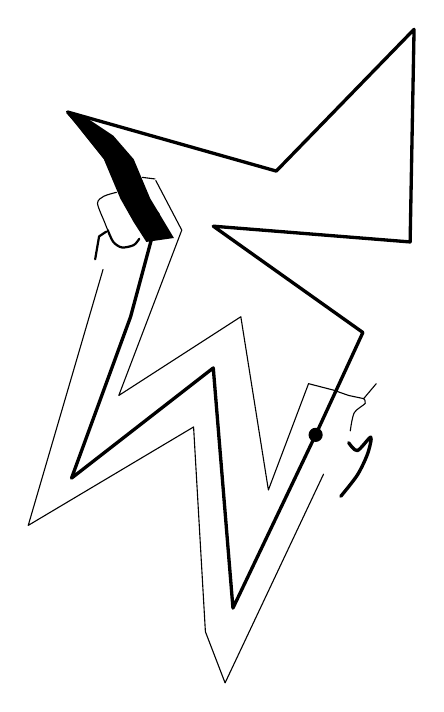
\begin{tikzpicture}[x=1mm,y=1mm,line cap=round,line join=round,font=\scriptsize]
\draw[very thick] (19.5,-24) -- (46,-31.5) -- (63.5,-13.5) -- (63,-40.5) -- (38,-38.5) -- (57,-52) -- (51,-65) -- (40.5,-87) -- (38,-56.5) -- (20,-70.5) -- (27.5,-50) -- (31,-37) -- cycle;
\draw (30.7,-32.7) -- (34,-39) -- (26,-60) -- (41.5,-50) -- (45,-72) -- (50.1,-58.5);
\draw (24,-44) -- (14.5,-76.5) -- (35.5,-64) -- (37,-90) -- (39.5,-96.5) -- (52,-70);
% the heavy left branch is a filled wedge on the page
\fill (19.4,-24.1) -- (21.7,-27) -- (24.1,-30) -- (26.2,-35) -- (27.9,-38) -- (29.5,-40.5) -- (33,-40) -- (30,-35) -- (27.9,-30) -- (25.3,-27) -- (22,-24.8) -- cycle;
% small loop of the thin line at the left of the wedge, with a short tick at its top right
\draw plot[smooth] coordinates {(25.7,-34.2) (24.1,-34.7) (23.3,-35.6) (24.2,-38) (24.6,-39)};
\draw[thick] plot[smooth] coordinates {(24.6,-39) (25.3,-40.5) (26.4,-41.2) (27.9,-40.9) (28.6,-40.1)};
\draw[thick] (24.4,-39.2) -- (23.5,-39.8) -- (23,-42.7);
\draw (29,-32.3) -- (30.6,-32.5);
% the strokes at the right, where the thin line ends: a cross stroke with a hook, a short stroke, a heavy hooked stroke; a blot on the heavy line
\draw (50.1,-58.5) -- (53.2,-59.3) -- (55.2,-60) -- (57.1,-60.4);
\draw plot[smooth] coordinates {(57.1,-60.4) (57.3,-61) (55.9,-62.2) (55.4,-64.5)};
\draw (57.1,-60.4) -- (58.7,-58.5);
\draw[very thick] plot[smooth] coordinates {(55.2,-66) (56.3,-67) (58,-65.3) (57.6,-67.4) (56.3,-70.1) (54.2,-72.8)};
\fill (51,-65) circle[radius=0.9];
\end{tikzpicture}
\end{document}
